% !TeX root = thesis.tex

\chapter{Approach}
\label{ch:approach}

This chapter details the methodology for automatically generating modality-grounded
question--answer (QA) annotations across multiple sensor modalities and
designing a benchmark to evaluate Vision-Language Models (VLMs). The proposed
system converts aligned, multi-sensor raw video streams into reliable,
modality-grounded QA pairs through a structured pipeline involving temporal
alignment, three-stage prompt chaining, fine-grained atomic splitting, LLM-assisted
semantic quality control, and late fusion with category-driven reliability filtering.
Finally, it establishes controlled benchmarking protocols to assess model robustness
under single-modality baseline, modality replacement, and native video input settings.

The pipeline distinguishes between two temporal alignment problems. First,
RGB, infrared, event, and depth representations from the same recording are
synchronized so that they describe the same physical events. Second, separately
captured daytime and nighttime recordings of the same activity are semantically
aligned because they may differ in duration, execution speed, pauses, and action
timing. This distinction enables controlled comparison across both sensor
modalities and illumination conditions.


\section{System Overview}
\label{sec:system_overview}

The primary goal of the annotation pipeline is to replace manual dataset
curation with an automated, multi-stage process that guarantees high data
quality, structural consistency, and verifiable grounding. Figure~\ref{fig:pipeline_overview}
illustrates the high-level architecture of the system.

\begin{figure}[ht]
    \centering
    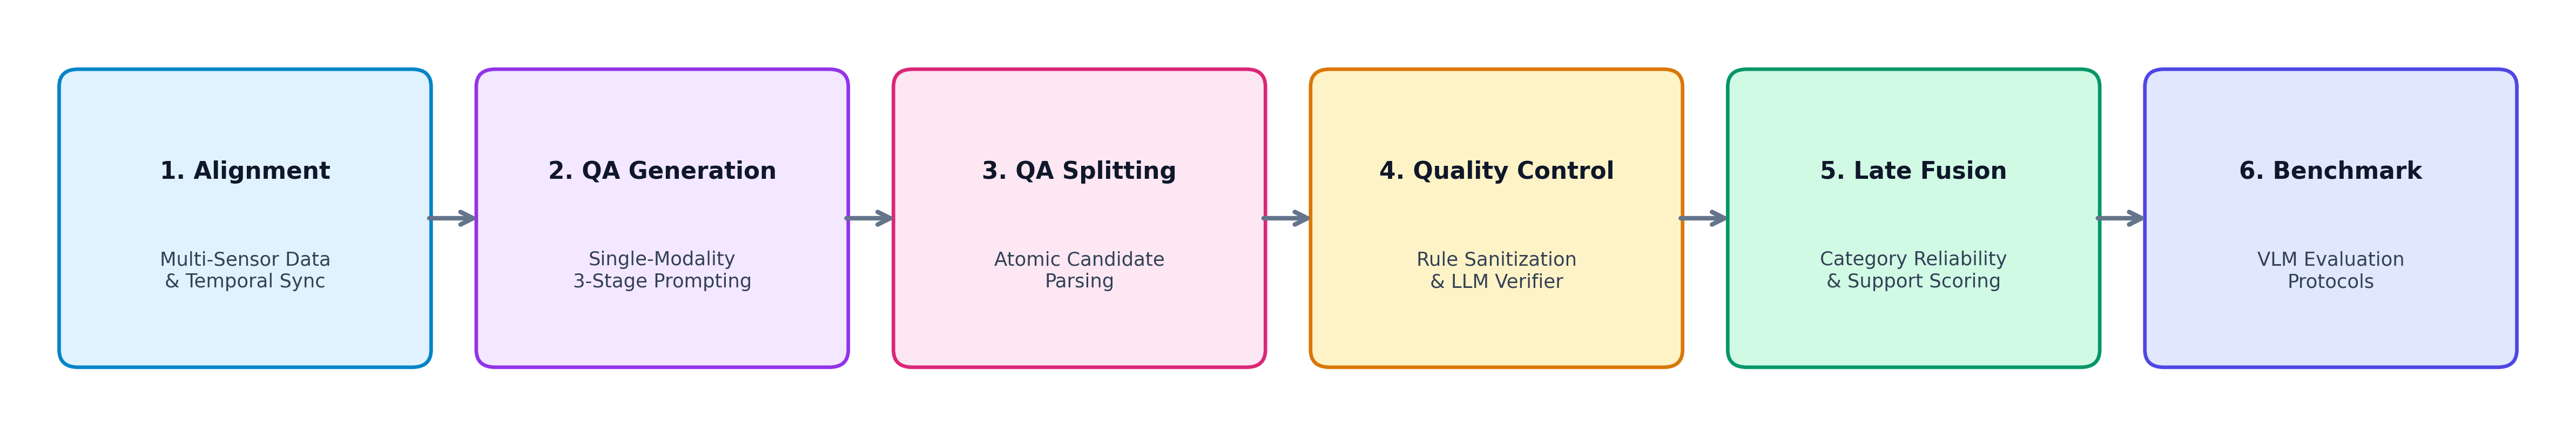
\includegraphics[width=\textwidth]{images/01_pipeline_overview.png}
    \caption{Overview of the automated multimodal annotation and benchmarking pipeline.}
    \label{fig:pipeline_overview}
\end{figure}

The pipeline operates in six main stages:
\begin{enumerate}
    \item \textbf{Data Preprocessing and Temporal Alignment:} Multi-sensor streams
          (RGB, Infrared, Event, and Marigold Depth) are synchronized using
          Dynamic Time Warping (DTW), cross-correlation, and optical flow, followed
          by task slicing and frame caching.
    \item \textbf{Single-Modality QA Generation:} Each modality is independently
          prompted using a three-stage chain (Captioning $\rightarrow$ Question Generation
          $\rightarrow$ Answering) powered by Gemini-based Large Language Models, tailored to modality-specific perception strengths.
    \item \textbf{Atomic QA Splitting:} Compound multi-question outputs generated by the LLMs
          are parsed and split into fine-grained atomic QA candidates.
    \item \textbf{Rule-Based and Semantic Quality Control:} Candidates are passed through
          rule-based sanity filters (removing irrecoverable format mismatches) and an LLM-assisted semantic verifier
          (using a highly efficient model like Gemini 3.1 Flash Lite) evaluating answerability, caption support, answer matching, single-question structure, modality appropriateness, and hallucination risk.
    \item \textbf{Late Fusion and Reliability Scoring:} Cleaned candidate QA items from all
          modalities are integrated under a category-driven reliability framework that
          computes fusion scores and relation-aware cross-modal support.
    \item \textbf{VLM Benchmark Protocol Construction:} Validated items are formatted into
          standardized benchmarking protocols (Source-Modality Baseline, Primary
          Modality-Replacement, and Native Video Adapter) evaluated with a blinded
          semantic judge and task-aware metrics.
\end{enumerate}


\section{Multimodal Data Preprocessing and Temporal Alignment}
\label{sec:preprocessing_alignment}

The raw dataset consists of synchronized recordings from multiple indoor and outdoor
perceptual sensors under varying lighting conditions (e.g., day/with-light and night/no-light).

\subsection{Input Modalities}

The pipeline integrates four distinct perceptual input modalities:
\begin{itemize}
    \item \textbf{RGB Video:} Standard visual context providing rich color, texture,
          fine appearance details, and readable text.
    \item \textbf{Infrared (IR) Video:} Thermal/infrared imaging that captures target
          structures and object silhouettes under low-light or zero-light conditions.
    \item \textbf{Event-Based Streams:} Asynchronous bio-inspired event data capturing
          high-temporal-resolution intensity changes, highlighting motion boundaries and fast dynamics.
    \item \textbf{Marigold Depth Maps:} Estimated monocular depth representations providing
          geometrical layout, spatial boundaries, and 3D structure.
\end{itemize}

\subsection{Temporal Synchronization}

Because different sensors operate at varying frame rates and output modalities,
temporal alignment is essential to ensure that visual evidence corresponds
to identical physical events:
\begin{itemize}
    \item \textbf{RGB--Event Alignment:} Dynamic Time Warping (DTW) aligns high-speed
          event accumulations with standard 30 FPS RGB video streams.
    \item \textbf{Day--Night Optical Flow Alignment:} Optical flow fields validate spatial
          and temporal alignment between paired day (with-light) and night (no-light) runs.
\end{itemize}

RGB is treated as the reference timeline for within-recording synchronization.
For each frame-based modality, a one-dimensional activity signal is extracted
from consecutive frames using grayscale differences or optical-flow magnitude.
For a target modality $m$ whose timing difference can be represented by a fixed
offset, normalized cross-correlation estimates the temporal displacement as

\begin{equation}
    \hat{\tau}_m =
    \underset{\tau}{\arg\max}
    \sum_t
    \tilde{x}_{\mathrm{rgb}}(t)
    \tilde{x}_m(t+\tau),
    \label{eq:cross_correlation_alignment}
\end{equation}

where $\hat{\tau}_m$ denotes the estimated temporal offset for target modality $m$, $\tau$ represents candidate time shifts, $t$ indexes temporal frames, and $\tilde{x}_{\mathrm{rgb}}$ and $\tilde{x}_m$ are normalized 1D activity signals for the reference RGB stream and target modality $m$, respectively. Intuitively, Equation~\ref{eq:cross_correlation_alignment} slides the target modality's motion activity signal along the RGB timeline and selects the time lag $\hat{\tau}_m$ that yields the maximum overlap in motion peaks, thereby correcting fixed hardware clock offsets between different sensors. The choice between alignment methods is governed by modality characteristics and residual drift checks: Cross-correlation is applied first to fixed-frame sensors (RGB, Infrared, Depth) sharing constant sampling rates, whereas Dynamic Time Warping (DTW) is deployed for asynchronous event streams or cross-run day--night alignments where non-linear speed variations and local temporal drift occur.

Daytime and nighttime recordings are aligned at the activity level rather than
through sensor-clock synchronization. Optical-flow activity is used to represent
motion correspondence, while a monotonic DTW mapping identifies matching
temporal positions across the two recordings. Unmatched introductory or trailing
regions are permitted when one recording contains additional activity.

\subsection{Task Slicing and Frame Caching}

Long recordings are partitioned into fixed 30-second synchronized segments (`task slicing`).
For efficient model processing, frames are uniformly sampled and cached at 1 FPS (producing approximately
30 frames per 30-second segment). For controlled eight-frame VLM benchmarking, a deterministic
sampling policy selects four frames from the day recording and four frames from the aligned night
recording for each segment.

The day--night alignment mapping is used to determine corresponding segment
boundaries, but it is not used to retime or reconstruct the benchmark videos.
The daytime and nighttime intervals are exported independently from their
original recordings. Consequently, each segment preserves its native frame
order, playback speed, motion characteristics, and frame rate while remaining
semantically paired through shared segment identifiers (\texttt{segment\_id}) and identical
underlying question items.

Each segment is assigned metadata containing its source recording, lighting
condition, start and end timestamps ($[t_{\mathrm{start}}, t_{\mathrm{end}}]$),
duration, and a corresponding day--night segment identifier. This metadata is
shared across all visual modalities so that questions, predictions, and
evaluation results can be traced back to the same underlying activity interval.


\section{Single-Modality QA Annotation Pipeline}
\label{sec:qa_generation_splitting}

To prevent LLM hallucinations and ensure that generated questions are strictly grounded
in visual evidence, QA generation follows a prompt-chained workflow per modality.

\subsection{Three-Stage Prompt Chain}

Instead of asking an LLM to generate QA pairs directly from raw video inputs in a single step,
the system executes a three-stage prompt chain:
\begin{enumerate}
    \item \textbf{Modality Captioning:} The model generates a detailed description focused
          on the specific perceptual strengths of the input modality (e.g., scene layout for RGB,
          motion contours for Event, spatial depth for Marigold).
    \item \textbf{Question Generation:} Operating on both the input frames and the generated
          caption, the model formulates questions designed to evaluate specific reasoning capabilities.
          Questions are prompted to ask from a first-person perspective (treating the subject as ``I'').
    \item \textbf{Answer Generation:} Given the input frames, caption, and formulated question,
          the model generates concise, unambiguous ground-truth answers.
\end{enumerate}

\subsection{Modality-Specific Task Categories}

Each modality is prompted with specialized task categories tailored to its physical domain:
\begin{itemize}
    \item \textbf{RGB:} \texttt{object\_recognition}, \texttt{spatial\_reasoning}, \texttt{text\_recognition},
          \texttt{scene\_sequence}, \texttt{light\_recognition}, \texttt{light\_change}, \texttt{counting}, \texttt{dynamic\_counting}, \texttt{non\_common}, \texttt{navigation}, \texttt{dynamic\_recognition}, and \texttt{action}.
    \item \textbf{Infrared (IR):} Uses the same 12 comprehensive task categories as RGB to enable matched evaluation.
    \item \textbf{Event:} \texttt{event\_object\_recognition}, \texttt{event\_spatial\_reasoning}, \texttt{event\_scene\_sequence},
          \texttt{event\_counting}, \texttt{event\_dynamic\_counting}, \texttt{event\_navigation}, \texttt{event\_dynamic\_recognition}, \texttt{event\_action}, and \texttt{event\_non\_common}.
    \item \textbf{Depth:} \texttt{depth\_object\_recognition}, \texttt{depth\_spatial\_reasoning}, \texttt{depth\_scene\_sequence},
          \texttt{depth\_counting}, \texttt{depth\_dynamic\_counting}, \texttt{depth\_navigation}, \texttt{depth\_dynamic\_recognition}, \texttt{depth\_action}, and \texttt{depth\_non\_common}.
\end{itemize}

The generated questions are also constrained not to reveal the experimental
condition through their wording. Expressions such as ``in the night video'',
``in the daytime scene'', or direct references to the source modality are
avoided unless the sensing condition itself is the subject of the question.
This prevents evaluated models from using linguistic shortcuts instead of
interpreting the provided visual evidence.

Where corresponding day and night evidence is available, the same question or
a semantically equivalent formulation is used for both conditions. The
reference answer remains tied to the underlying activity rather than to the
lighting label, enabling a direct comparison of model behaviour across day and
night inputs.

\subsection{Atomic QA Splitting}

Initial outputs from LLM generation often return compound blocks where a single response contains
several numbered questions and answers. Evaluating compound blocks directly introduces ambiguity.
The pipeline extracts every individual question--answer pair, parsing 2,730 raw generated blocks
into 7,310 atomic QA candidate items. Each atomic item receives a standardized structure containing an
\texttt{annotation\_key}, \texttt{category}, source \texttt{modality}, question text, reference answer,
and parent block metadata.


\section{Rule-Based and LLM-Assisted Quality Control}
\label{sec:quality_control}

Prior to late fusion, atomic QA candidates undergo a two-tier quality control pipeline to remove malformed and nonsensical generation artifacts.

\subsection{Rule-Based Filtering}

Initial rule-based sanitization eliminates malformed data by checking:
\begin{itemize}
    \item Mismatches between question and answer counts.
    \item Presence of explicit frame number references in question text (e.g., ``In frame 12, what...'').
    \item Abnormally short, empty, or duplicate responses.
    \item Unresolved formatting syntax.
\end{itemize}
Out of 2,730 raw blocks, 1,263 passed directly, 614 were transformed, and 853 generated warnings. This process removed 9 irrecoverable candidates, passing 7,301 atomic candidates to the semantic verifier.

\subsection{LLM-Assisted Semantic Verification}

The remaining atomic candidates are evaluated by an LLM-assisted semantic verifier (using Gemini 3.1 Flash Lite) across five binary dimensions and one risk dimension:
\begin{enumerate}
    \item \textbf{Answerability:} Verifies that the question can be answered from visual evidence.
    \item \textbf{Answer Matching:} Checks whether the generated answer accurately and directly addresses the question.
    \item \textbf{Caption Support:} Confirms that the answer is explicitly supported by the modality caption.
    \item \textbf{Modality Appropriateness:} Checks whether the target question aligns with the physical capabilities of the source modality.
    \item \textbf{Single Question Structure:} Ensures the item is not a compound question.
    \item \textbf{Hallucination Risk:} Estimates the risk of non-grounded inferences (\texttt{low}, \texttt{medium}, or \texttt{high}).
\end{enumerate}

Of the 7,301 evaluated atomic candidates, the verifier passed 5,916 (81.0\%), marked 507 for review (6.9\%), and rejected 878 (12.0\%).


\section{Late Fusion and Category-Driven Reliability Verification}
\label{sec:late_fusion_reliability}

The late fusion module integrates the cleaned modality-specific QA candidates into a unified dataset.
Its design is governed by the core principle:
\begin{center}
    \textit{``Category controls reliability; section controls evaluation grouping.''}
\end{center}
The category assigned during single-modality generation dictates scoring and filtering rules,
whereas section labels govern how QA items are grouped for VLM capability evaluation.

\subsection{Fusion Score Formulation}

For each QA candidate, a composite fusion score $S_{\text{fusion}}$ conceptually estimates overall reliability:
\begin{equation}
    S_{\text{fusion}} = w_{\text{modality}}(\text{cat}, m) \cdot S_{\text{validity}} \cdot S_{\text{atomic}} + \alpha \cdot S_{\text{support}},
    \label{eq:fusion_score}
\end{equation}
where $S_{\text{fusion}}$ represents the overall composite fusion score, $w_{\text{modality}}(\text{cat}, m) \in [0, 1]$ assigns category-specific domain confidence weights to source modality $m$ under task category $\text{cat}$, $S_{\text{validity}} \in \{0, 1\}$ indicates structural completeness, $S_{\text{atomic}} \in \{0, 1\}$ rewards cleanly split single-question items, $S_{\text{support}} \in [0, 1]$ measures cross-modal evidence agreement, and $\alpha$ is a hyperparameter balancing single-modality validity against cross-modal verification.

\subsection{Relation-Aware Cross-Modal Support}

To compute $S_{\text{support}}$, candidate evidence is matched against descriptions from other modalities.
Rather than treating all matching text as equal, the system classifies cross-modal relations into four categories:
\begin{enumerate}
    \item \textbf{Direct Support ($\text{rel} = \text{direct}$):} Strong lexical and semantic alignment from a compatible modality (e.g., IR supporting RGB object presence).
    \item \textbf{Complementary Support ($\text{rel} = \text{complementary}$):} Partial or indirect evidence from a secondary modality (e.g., Event supporting RGB action).
    \item \textbf{Conflict ($\text{rel} = \text{conflict}$):} Contradictory evidence (e.g., direction, negation, or count discrepancies).
    \item \textbf{Weak or Irrelevant ($\text{rel} = \text{weak}$):} Insufficient overlap or incompatible modality combination.
\end{enumerate}
The cross-modal support score is conservatively defined as:
\begin{equation}
    S_{\text{support}} = \max\left(S_{\text{direct}},\, 0.5 \cdot S_{\text{complementary}}\right),
    \label{eq:support_score}
\end{equation}
where $S_{\text{direct}}$ and $S_{\text{complementary}}$ denote the semantic evidence agreement scores obtained from direct and complementary supporting modalities, respectively.

\subsection{Category Gates and Review Queue}

Candidates pass through category-specific filtering gates:
\begin{itemize}
    \item \texttt{support\_required}: Mandatory direct cross-modal verification (e.g., object recognition, counting, spatial reasoning).
    \item \texttt{support\_soft}: Cross-modal support is beneficial but optional (e.g., action, motion, dynamic recognition).
    \item \texttt{support\_exempt}: Single-modality dependencies allowed (e.g., text recognition).
    \item \texttt{review\_recommended}: Anomaly or non-standard items sent to an automated review queue.
\end{itemize}

Items flagged with potential issues (e.g., low lexical overlap despite high semantic similarity, multi-clause answers,
or numeric/directional conflicts) are placed in a prioritized review queue (\texttt{high}, \texttt{medium}, or \texttt{low} priority) for inspection.
The final retention stage retains 5,465 valid QA items that comprise the visual VLM benchmark.


\section{VLM Benchmark Design and Evaluation Protocols}
\label{sec:benchmark_protocols}

To systematically evaluate Vision-Language Models on the generated dataset, three benchmark protocols are established.

\subsection{Source-Modality Baseline Protocol}

The source-modality baseline evaluates all 5,465 visual QA items using the exact visual modality from which each question was generated (2,318 RGB, 1,561 IR, 822 Event, and 764 Depth). This experiment verifies whether retained items remain answerable under their intended evidence source and establishes upper-bound model performance.

\subsection{Primary Modality-Replacement Protocol}

To measure model robustness against visual representation changes without changing the underlying reasoning task, the primary benchmark uses a same-question modality-replacement setup.
From the dataset, 5,331 questions are identified for which aligned RGB, Infrared, Event, and Depth representations are simultaneously available. Each question is independently evaluated four times under each visual modality:
\begin{equation}
    N_{\text{total\_evals}} = 5,331 \text{ questions} \times 4 \text{ modalities} = 21,324 \text{ evaluations per model}.
\end{equation}
This balanced, paired setup isolates visual representation robustness from question difficulty.

\subsection{Visual Input Representations: Fixed 8-Frame vs. Native Video}

Model evaluation is conducted under two distinct input representations:
\begin{itemize}
    \item \textbf{Fixed 8-Frame Protocol:} All models receive identical visual evidence consisting of eight deterministically sampled frames (4 day/light frames + 4 night/dark frames). Decoding parameters, temperature, and frame order are fixed across all models.
    \item \textbf{Native Video Adapter Protocol:} Full aligned video files are passed through each model's native video adapter, allowing family-specific frame sampling, tokenization, and temporal aggregation.
\end{itemize}

\subsection{Evaluation Metrics}

Evaluation relies on a combination of semantic LLM judging and automated task-aware metrics:
\begin{itemize}
    \item \textbf{Blinded Semantic Judge:} A blinded LLM judge classifies model answers into \texttt{correct} (1.0), \texttt{partially\_correct} (0.5), \texttt{incorrect} (0.0), or \texttt{unjudgeable} (excluded). Strict accuracy ($\mathrm{Acc}_{\mathrm{strict}}$) and Soft accuracy ($\mathrm{Acc}_{\mathrm{soft}}$) are defined as:
          \begin{equation}
              \mathrm{Acc}_{\mathrm{strict}} = \frac{N_{\mathrm{correct}}}{N_{\mathrm{correct}} + N_{\mathrm{partial}} + N_{\mathrm{incorrect}}},
          \end{equation}
          \begin{equation}
              \mathrm{Acc}_{\mathrm{soft}} = \frac{N_{\mathrm{correct}} + 0.5 N_{\mathrm{partial}}}{N_{\mathrm{correct}} + N_{\mathrm{partial}} + N_{\mathrm{incorrect}}}.
          \end{equation}
    \item \textbf{Task-Aware Automated Metrics:} Deterministic metrics complement the judge based on QA task category: Boolean Accuracy for yes/no, Numeric Accuracy for counting, ANLS for text/OCR, Sequence-Order Score for temporal tasks, Set F1 for multi-concept answers, and Token F1 for open-ended questions.
\end{itemize}


\section{Contrastive Day--Night Analysis}
\label{sec:contrastive_day_night}

In addition to aggregate accuracy, model performance is analyzed separately for
semantically corresponding daytime and nighttime inputs. Let $c_d$ and $c_n$
represent binary correctness for the daytime and nighttime versions of a QA
item, respectively. Each paired result is assigned to one of four outcomes:

\begin{equation}
    (c_d,c_n)
    \in
    \left\{
        (1,0),\,
        (0,1),\,
        (1,1),\,
        (0,0)
    \right\}.
    \label{eq:day_night_outcomes}
\end{equation}

The four outcomes correspond to
\textit{day-pass/night-fail},
\textit{night-pass/day-fail},
\textit{both-pass}, and
\textit{both-fail}. A day-pass/night-fail result indicates that the model
benefits from daytime visibility, whereas a night-pass/day-fail result suggests
that nighttime-specific cues or a non-RGB sensor representation provide more
useful evidence. Both-pass cases indicate robustness across illumination
conditions, while both-fail cases identify questions that are difficult or
ambiguous under both conditions.

This contrastive analysis is performed separately for RGB, infrared, event, and
depth inputs. It therefore measures not only general illumination robustness,
but also whether the usefulness of a sensor changes between daytime and
nighttime conditions. The analysis prevents overall accuracy from hiding
asymmetric failures that occur predominantly under one illumination setting.


\section{Summary}
\label{sec:approach_summary}

This chapter presented an end-to-end framework for multimodal QA annotation and VLM benchmarking. By combining temporal alignment across four modalities, a three-stage prompt chain, atomic QA splitting, late fusion with relation-aware support scoring, and two-tier quality control, the pipeline retains 5,465 high-quality QA items from raw multi-sensor streams. The resulting benchmark protocols (Source-Modality Baseline, Modality Replacement, and Native Video Adapter) enable rigorous, controlled evaluation of VLM capabilities across diverse visual representations.